%----------------------------------------------------------------------------------------
%	PACKAGES AND OTHER DOCUMENT CONFIGURATIONS
%----------------------------------------------------------------------------------------

\documentclass[letterpaper,twoside,11pt]{article}

%% Jose Javier Gonzalez Ortiz %%
%% Plantilla Latex generica   %%
%% 2014-11-08                 %%

\usepackage{lipsum} % Package to generate dummy text throughout this template

\usepackage[sc]{mathpazo} % Use the Palatino font
\usepackage[T1]{fontenc} % Use 8-bit encoding that has 256 glyphs
\linespread{1.05} % Line spacing - Palatino needs more space between lines
\usepackage{microtype} % Slightly tweak font spacing for aesthetics

\usepackage[letterpaper,hmarginratio=1:1,top=32mm,left=20mm,right=20mm,columnsep=20pt]{geometry} % Document margins
\usepackage{multicol} % Used for the two-column layout of the document
\usepackage[hang, small,labelfont=bf,up,textfont=it,up]{caption} % Custom captions under/above floats in tables or figures
\usepackage{booktabs} % Horizontal rules in tables
\usepackage{float} % Required for tables and figures in the multi-column environment - they need to be placed in specific locations with the [H] (e.g. \begin{table}[H])
\usepackage{hyperref} % For hyperlinks in the PDF

\usepackage{lettrine} % The lettrine is the first enlarged letter at the beginning of the text
\usepackage{paralist} % Used for the compactitem environment which makes bullet points with less space between them

\usepackage{abstract} % Allows abstract customization
\renewcommand{\abstractnamefont}{\normalfont\bfseries} % Set the "Abstract" text to bold
\renewcommand{\abstracttextfont}{\normalfont\small\itshape} % Set the abstract itself to small italic text

\usepackage{titlesec} % Allows customization of titles
% \renewcommand\thesection{\Roman{section}} % Roman numerals for the sections
% \renewcommand\thesubsection{\Roman{subsection}} % Roman numerals for subsections
\titleformat{\section}[block]{\large\scshape\centering}{\thesection.}{1em}{} % Change the look of the section titles
\titleformat{\subsection}[block]{\large}{\thesubsection.}{1em}{} % Change the look of the section titles

\usepackage{fancyhdr} % Headers and footers


\usepackage{indentfirst}

% Generic Pakages
    \usepackage[utf8]{inputenc}                         % For Spanish characters
    \usepackage[english]{babel}               % Spanish hyphenation and document rules
    \usepackage{amsmath}                                % Standard math packages
    \usepackage{graphicx}                               % Image insertion.
    \usepackage{tikz}
    \usepackage{caption,subcaption}                     % For custom caption environments

    

    \usepackage{appendix}                               % Enables appendices
    \usepackage{pdfpages}                               % Insert pdfs
    \usepackage{array}                                  % Enables array features
    \usepackage{algorithm}
    \usepackage[noend]{algpseudocode}
    \usepackage{eqparbox}
    \makeatletter
    \def\BState{\State\hskip-\ALG@thistlm}
    \makeatother
    %\usepackage[americanvoltages, europeancurrents, americanresistors, cuteinductors]{circuitikz}                          % Circuit Graphics
    \usepackage{mathtools}
    \usepackage{amsthm}
    
%Additional Features
    
    \usepackage{enumerate}                              % Custom numerate, useful for i,ii,iii... I,II,III...
    \usepackage{sectsty}                                % Allows customizing section commands
    \usepackage{todonotes}                              % useful for leaving todonotes
    \usepackage[space]{grffile}                         % insert files with spaces
     %\usepackage{microtype}                             % Beatify engine
    %\usepackage[superscript]{cite}                     % CIting with superscript numerals
    %\usepackage{xcolor}                                    % Required for inserting color
    %\usepackage[usenames,dvipsnames]{color}                % Required for custom colors
    %\usepackage{xargs}                                 % Expanded arguments features
    %\usepackage{fix-cm}                                 % Computer-Modern at arbitrarysizes
    \usepackage{siunitx}                               % For SI Units
    %\usepackage{eurosym}                                % Eurosymbol
    %\usepackage{pdflscape}                              % enables landscape for pdfs
    %\usepackage{longtable}                              % Tables than span multipages

% Custom Settings
    % \decimalpoint                                       % American Decimal Point instead of Spanish comma

    % Margins
    %     \topmargin      = -0.45in
    %     \evensidemargin = 0in
    %     \oddsidemargin  = 0in
    %     \textwidth      = 6.5in
    %     \textheight     = 9.0in
    %     \headsep        = 0.25in

    % \pagestyle{fancy}
    % \lhead{\HWAuthorName}
    % \chead{}
    % \rhead{\HWClass : \HWTitle}
    % \lfoot{}
    % \cfoot{\thepage}
    % \rfoot{}
    
    % \renewcommand\headrulewidth{0.4pt} % Size of the header rule
    % \renewcommand\footrulewidth{0.4pt} % Size of the footer rule

    \numberwithin{equation}{section} % Number equations within sections (i.e. 1.1, 1.2, 2.1, 2.2 instead of 1, 2, 3, 4)
    \numberwithin{figure}{section} % Number figures within sections (i.e. 1.1, 1.2, 2.1, 2.2 instead of 1, 2, 3, 4)
    \numberwithin{table}{section} % Number tables within sections (i.e. 1.1, 1.2, 2.1, 2.2 instead of 1, 2, 3, 4)

    \renewcommand{\labelitemi}{$\bullet$}                       %%bullet1 circle
    \renewcommand{\labelitemii}{\leavevmode \hbox to
    1.2ex {\hss \vrule height .9ex width .7ex depth -.2ex\hss }} %%bullet2 box

    \newcommand{\ul}[1]        {\underline{\smash{#1}}}         %%closer underline
    \newcommand{\gm}[1]         {\guillemotleft #1\guillemotright}  %$ pretty <<sth>>$

    \DeclarePairedDelimiter\floor{\lfloor}{\rfloor}
    \DeclarePairedDelimiter\ceil{\lceil}{\rceil}

%%%%%%%%%%%%%%%%%%%%%%%%%%%%%%%%%%%%%%%%%%%%%%%%%%%%%%%%%%%%%%%%%%%%%%%%%%%%%%%%%%
%%%                             CODIGO                                         %%%
%%%%%%%%%%%%%%%%%%%%%%%%%%%%%%%%%%%%%%%%%%%%%%%%%%%%%%%%%%%%%%%%%%%%%%%%%%%%%%%%%%

% Code insertion
    \usepackage{listings}                               % Main package for inserting code
    \usepackage{courier}                                % For using the courier font

    \AtBeginDocument{\numberwithin{lstlisting}{section}}  % Number listings within sections (i.e. 1.1, 1.2, 2.1, 2.2 instead of 1, 2, 3, 4)
    
    %%\captionsetup[lstlisting]{font={small,tt}}            %  Listings Font Size
    
    % \renewcommand{\lstlistingname}{Código}              % For Codigo caption (requires caption package)

    \definecolor{background}{gray}{.98}                 % Background color definition
    \definecolor{comments}{RGB}{51,102,0}               % Comments   color definition
    \definecolor{keywords}{RGB}{0,0,120}                % Keywords   color definition
    \definecolor{keywords2}{RGB}{204,0,102}             % Keywords2  color definition
    \definecolor{numbers}{RGB}{127, 0, 127}             % Keywords2  color definition

    \definecolor{Maroon}{RGB}{128, 0, 0}

       % morekeywords={add,sub,mul,mulu,nand,sll,sra,srl,sltu,addi,sw,lw,beq,jarl,lui},
    \lstdefinelanguage{ICAI-RiSC-16}
   {morekeywords={add,sub,mul,mulu,nand,sll,sra,srl,sltu,addi,sw,lw,beq,jalr,lui,la,med},
        sensitive=false,
        morecomment=[l]{\#},
        morecomment=[l][\color{Maroon}]{.},
        morekeywords=[2]{r0, r1, r2, r3, r4, r5, r6, r7},
        keywordstyle=[2]{\color{violet}},
        % literate=%
        %    *{0}{{{\color{red!20!violet}0}}}1
        %     {1}{{{\color{red!20!violet}1}}}1
        %     {2}{{{\color{red!20!violet}2}}}1
        %     {3}{{{\color{red!20!violet}3}}}1
        %     {4}{{{\color{red!20!violet}4}}}1
        %     {5}{{{\color{red!20!violet}5}}}1
        %     {6}{{{\color{red!20!violet}6}}}1
        %     {7}{{{\color{red!20!violet}7}}}1
        %     {8}{{{\color{red!20!violet}8}}}1
        %     {9}{{{\color{red!20!violet}9}}}1
        %morecomment=[s]{/*}{*/},
        %morestring=[b]"
    }


    \lstset{
        frame=Ltb,
        framerule=0pt,
        aboveskip=0.5cm,
        framextopmargin=3pt,
        framexbottommargin=3pt,
        framexleftmargin=0.4cm,
        framesep=0pt,
        rulesep=.4pt,
        backgroundcolor=\color{background},
        rulesepcolor=\color{black},
        rulecolor=\color{black},
        %
        stringstyle=\ttfamily,
        basicstyle=\small\ttfamily,
        commentstyle=\itshape\color{comments},
        keywordstyle=\bfseries\color{keywords},
        %
        numberstyle=\tiny,
        numbers=left,
        numbersep=15pt,
        numberfirstline = false,
        %
        breakatwhitespace=false,         % sets if automatic breaks should only happenat whitespace
        breaklines=true,                 % sets automatic line breaking
        captionpos=b,                    % sets the caption-position to bottom
        escapeinside={<@}{@>},            % if you want to add LaTeX within your code
        keepspaces=true,                 % keeps spaces in text, useful for keepingindentation of code (possibly needs columns=flexible)
        showspaces=false,                % show spaces everywhere adding particularunderscores; it overrides 'showstringspaces'
        showstringspaces=false,          % underline spaces within strings only
        showtabs=false,                  % show tabs within strings adding particularunderscores
        stepnumber=1,                    % the step between two line-numbers. If it's1, each line will be numbered
        tabsize=2,                       % sets default tabsize to 2 spaces
    }
    

    \lstdefinestyle{customvhdl}{
        language=vhdl,                              % Language
        morekeywords = {},
        morestring=[b][\color{numbers}]',
        morestring=[b][\color{numbers}]",
        emph={std_logic,std_logic_vector,integer,unsigned,to_unsigned},
        emphstyle={\color{keywords2}\bfseries},%
        %deletekeywords={...},            % if you want to delete keywords from the given language
    }

    \lstdefinestyle{customcpp}{
        language = C++,
       %  directivestyle={\color{black}}
       % emph={int,char,double,float,unsigned},
       % emphstyle={\color{blue}}
    }

    \lstset{style = customcpp}



    % Grey scale definitions - Printing
    %\definecolor{background}{gray}{.98}
    %\definecolor{comments}{gray}{.45}
    %\definecolor{keywords}{gray}{.25}


%%%%%%%%%%%%%%%%%%%%%%%%%%%%%%%%%%%%%%%%%%%%%%%%%%%%%%%%%%%%%%%%%%%%%%%%
%%%%%%%%%%%%%%%%%%%%%%       HERE BE DRAGONS        %%%%%%%%%%%%%%%%%%%%
%%%%%%%%%%%%%%%%%%%%%%%%%%%%%%%%%%%%%%%%%%%%%%%%%%%%%%%%%%%%%%%%%%%%%%%%
%
%%%%%%%%%%%%%%%%%%%%%%%%%%%%%%%%%%%%%%%%%%%%%%%%%%%%%%%%%%%%%%%%%%%%%%%%
%%%% Paragraph separation
%\setlength{\parskip}{.5em}
%%%%%%%%%%%%%%%%%%%%%%%%%%%%%%%%%%%%%%%%%%%%%%%%%%%%%%%%%%%%%%%%%%%%%%%%
%%%% Table separation
%\renewcommand{\arraystretch}{1.3}
%%%%%%%%%%%%%%%%%%%%%%%%%%%%%%%%%%%%%%%%%%%%%%%%%%%%%%%%%%%%%%%%%%%%%%%%
%%%% 9+ Arguments functions
%\newcommand{\function}[9]{%
%        \def\tempa{#1}%
%        \def\tempb{#2}%
%        \def\tempc{#3}%
%        \def\tempd{#4}%
%        \def\tempe{#5}%
%        \def\tempf{#6}%
%        \def\tempg{#7}%
%        \def\temph{#8}%
%        \def\tempi{#9}%
%        \functioncont
%    }
%%%%%%%%%%%%%%%%%%%%%%%%%%%%%%%%%%%%%%%%%%%%%%%%%%%%%%%%%%%%%%%%%%%%%%%%
%%%% Rules for longtable
%\newcommand{\mytoprule}{\specialrule{1.5pt}{0em}{0em}}
%\newcommand{\mymidrule}{\specialrule{.75pt}{0em}{0em}}
%\newcommand{\mybottomrule}{\specialrule{1.5pt}{0em}{0em}}
%
%%%%%%%%%%%%%%%%%%%%%%%%%%%%%%%%%%%%%%%%%%%%%%%%%%%%%%%%%%%%%%%%%%%%%%%%
%%%% Roman numerals at the start
%
%\pagenumbering{roman}
%\tableofcontents
%\newpage
%\listoftables
%\newpage
%\pagenumbering{arabic}
%%%%%%%%%%%%%%%%%%%%%%%%%%%%%%%%%%%%%%%%%%%%%%%%%%%%%%%%%%%%%%%%%%%%%%%%
%%%% More than 18 floating figures/tables - force to put
%\clearpage
%%%%%%%%%%%%%%%%%%%%%%%%%%%%%%%%%%%%%%%%%%%%%%%%%%%%%%%%%%%%%%%%%%%%%%%%
%%%% Landscape tables recommendations
%\topmargin      = -0.95in
%\evensidemargin = 0in
%\oddsidemargin  = 0in
%\textwidth      = 6.5in %6.5in
%\textheight     = 9.75in
%\headsep        = 0.25in
%\small  % Switch from 12pt to 11pt
%\setlength\LTleft{0pt}            % default: \parindent
%\setlength\LTright{0pt}           % default: \fill
%%%%%%%%%%%%%%%%%%%%%%%%%%%%%%%%%%%%%%%%%%%%%%%%%%%%%%%%%%%%%%%%%%%%%%%%
%%%% Bold columns table
%>{\bfseries\arraybackslash}m{1.1in}
%
%%%%%%%%%%%%%%%%%%%%%%%%%%%%%%%%%%%%%%%%%%%%%%%%%%%%%%%%%%%%%%%%%%%%%%%%
%%%% \epigraph{}
%
%\makeatletter
%\patchcmd{\epigraph}{\@epitext{#1}}{\itshape\@epitext{#1}}{}{}
%\makeatother
%%%%%%%%%%%%%%%%%%%%%%%%%%%%%%%%%%%%%%%%%%%%%%%%%%%%%%%%%%%%%%%%%%%%%%%%
%%%% Quotes -> chapquote enviroment
%\makeatletter
%\newenvironment{chapquote}[2][2em]
%  {\setlength{\@tempdima}{#1}%
%   \def\chapquote@author{#2}%
%   \parshape 1 \@tempdima \dimexpr\textwidth-2\@tempdima\relax%
%   \itshape}
%  {\par\normalfont\hfill--\ \chapquote@author\hspace*{\@tempdima}\par\bigskip}
%\makeatother
%%%%%%%%%%%%%%%%%%%%%%%%%%%%%%%%%%%%%%%%%%%%%%%%%%%%%%%%%%%%%%%%%%%%%%%%

\pagestyle{fancy} % All pages have headers and footers
\fancyhead{} % Blank out the default header
\fancyfoot{} % Blank out the default footer
\fancyhead[L]{Jose Javier Gonzalez Ortiz}
\fancyhead[R]{EECS 587 : Parallel Computing} % Custom header text
\fancyfoot[RO,LE]{\thepage} % Custom footer text


\setlength{\parskip}{2mm}
\setlength{\headheight}{13.6pt}
%----------------------------------------------------------------------------------------
%	TITLE SECTION
%----------------------------------------------------------------------------------------

\title{\vspace{-15mm}\fontsize{24pt}{10pt}\selectfont\textbf{Parallel Implementation of Multiple Interdependent Lindenmayer Systems}} % Article title

\author{
\large
\textsc{Jose Javier Gonzalez Ortiz}\thanks{\href{mailto:jjgo@umich.edu}{jjgo@umich.edu}}\\[2mm] % Your name
\normalsize University of Michigan \\ % Your institution
% \normalsize \href{mailto:jjgo@umich.edu}{jjgo@umich.edu} % Your email address
% \vspace{-5mm}
}
\date{\today}

%----------------------------------------------------------------------------------------

\begin{document}

\maketitle % Insert title

\thispagestyle{fancy} % All pages have headers and footers

%----------------------------------------------------------------------------------------
%	ABSTRACT
%----------------------------------------------------------------------------------------

\begin{abstract}

\noindent \lipsum[1] % Dummy abstract text

\end{abstract}

%----------------------------------------------------------------------------------------
%	ARTICLE CONTENTS
%----------------------------------------------------------------------------------------

\begin{multicols}{2} % Two-column layout throughout the main article text

\section{Introduction}
% \vspace{-6mm}
\lettrine[nindent=0em,lines=2]{M}
odern techniques for botanic and arboreal growth simulation rely in specific and dedicated models to correctly recreate the behavior of different types of plants. This creates a segmented and disconnected variety of models and techniques. As A. Lindenmayer and Przemyslaw described in \cite{Prusinkiewicz:1996:ABP:235579}, almost all botanical structures can be successfully modeled by the so called Lindenmayer Systems.

However, raw L-Systems are not complex enough for this task and therefore we need to include a parametric implementation to successfully model these types of structures. Moreover, parametric L-Systems in spite of depending on a number of initial parameters and conditions, they portray a deterministic behavior. To cope with this limitation, we introduce randomness in the traditional form described in \cite{Prusinkiewicz:1996:ABP:235579}, by using Stochastic-Parametric L-Systems. These systems will have production rules that will not only rely on several parameters to correctly scalate the complexity of the system but will also apply this rules using a source of randomness to choose between a number of specified rules.

Another aspect we have to properly take into a account is the fact that botanical growth almost never occurs in a isolated fashion, and therefore we will be interested in looking at a framework that can accommodate the simultaneous derivation of multiple L-Systems. Having multiple stochastic L-Systems produces a non-realistic result as we will see later, so to compensate for this caveat we had to define the concept of Interdependent L-Systems.

In this paper we investigate the use of Interdependent L-System to realistically model the growth of a forest and we analyze several parallel implementations of this problem in a shared memory machine using OpenMP. L-Systems are parallel rewriting grammar which initially would seem to simplify the problem, but this derivation step leads to highly uneven amounts of work in a great number of scenarios. Furthermore, as we shall see later, adding the interdependence to the systems serializes the problem greatly, since after every timestep each system will need to communicate a number of metrics to a variable number of neighboring systems. This problem will produce a scenario experienced by a great amount of local simulation techniques.

We will introduce several parallel algorithms with increasing complexity and with increasing speedup and compare their behavior under different types of datasets, which from a simulation perspective would translate into different ecosystems. The final algorithm will involve calculating the connected components of the forest graph to initially subdivide the problem in equally complex albeit not equally balanced subproblems, and introduce a general approach to tackle this subproblems. To accomplish this, the algorithm will deserialize the time dimension by allowing some L-Systems to carry out further iterations as long as the correctness constraints are met. We will also analyze the bigger bottleneck of the algorithm and the way it tries to cope with the variability of input systems.

\textbf{Overview:} First  we will start by providing a background in canonical, parametric and stochastic L-Systems in Section \ref{sec:background}. Section \ref{sec:interdependence} will elaborate the model used to realistically simulate the problem and will discuss the serial implementation that was carried out. The parallel algorithms designed to solve this problem are discussed in Section \ref{sec:parallelization} and their associated results are shown in Section \ref{sec:results} and analyzed in Section \ref{sec:discussion}.

\subsection{Previous Work} % (fold)
\label{sub:previous_work}
\textbf{General L-Systems:} Prusinkiewicz and Lindenmayer gave the basic definition to the L-System algorithm and structure in \cite{Prusinkiewicz:1996:ABP:235579}. This was further extended by the work carried out in \cite{Parish:2001:PMC:383259.383292,Prusinkiewicz:1994:ST:192161.192254,Prusinkiewicz:2001:UPI:383259.383291}

\textbf{Parallelizing L-Systems:} Lacz and Hart introduced the use of manually written pixel shaders to compute L-Systems \cite{Lacz04proceduralgeometry}. A distributed memory approach making use up to 8 CPUs and the Message Passing Interface (MPI) was described in \cite{4392608}. An algorithm form the Parallel Generation of L-Systems was introduced by \cite{LIPP-2009-PGL}. The approach was appropriate for both GPU and multi-core CPUs, parallelizing both the derivation and interpretation of given L-Systems. The implementation provided was generic and supported parametric, stochastic and context sensitive productions. The work was further extended in \cite{LIPP-2010-PGMS} to make the algorithm work with multiple L-Systems.

\textbf{Forest Simulation:} L-Systems are within the most popular grammars to satisfactory model botanical structures. The definitions introduced by \cite{Prusinkiewicz:1996:ABP:235579} were later improved to more realistic three dimensional trees in \cite{4055766}. Since then, both models have been used in a number of forest growth models.

The model proposed by \cite{KurthSloboda2002} provides a wonderful framework to model the interdependence of L-Systems. Geometrical interpretation of parameters was used to calculate shadow cones and a carbon allocation economy was used to successfully control the growth of the trees. A later paper introduced a quasi-physical simulation of large-scale dynamic forest scenes by introducing a similar growth model and a wind field to account for environmental factors. Finally, \cite{Runions07modelingtrees} introduced a new model by employing a three dimensional version of the space colonization algorithm.
% subsection previous_work (end)

%------------------------------------------------

\section{Background} % (fold)
\label{sec:background}

\subsection{Definition} % (fold)
\label{sub:definition}

The work presented in this paper is based on L-systems so we will briefly introduce this modeling structure.

\emph{L-Systems:} are parallel rewriting systems and a type of formal grammar. L-systems are now commonly referred as \emph{parametric} L-systems, defined as a tuple:
\begin{equation}
	\textbf{G} = (V, \omega, P)
\end{equation}
where
\begin{compactitem}
\item $\textbf{V}$ (\emph{alphabet}) is a set of symbols containing the elements in the string that can be replaced.
\item $\boldsymbol\omega$ (\emph{axiom}) is a string of symbols from $V$ defining the initial state of the system.
\item $\textbf{P}$ is a set of \emph{production rules} which define the way variables can be replaced with combinations of constants and variables. Each rule is composed by a \emph{predecessor} and a \emph{successor}. The successor will consist of a list of symbols that will replace the predecessor. Usually the predecessor contains only one symbol, if it involves more, the system is called \emph{context sensitive}. If a production rule is not specified for a symbol, the identity production is assumed.
\end{compactitem}

\emph{Parametric L-systems:} We can further expand the definition of L-system to accommodate parameters. In a parametric grammar, each symbol in the alphabet has a list of parameters associated with it. Parameters are usually real valued but there is not constraint in the mathematical structures that can be used. Production rules need to be extended to deal with parametric symbols. Parameters can be both \emph{global} or \emph{local} depending on if they belong to the current predecessor. Parameters are used in both conditional statements to choose between different production rules and for modifying the parameters of the symbols in the successor.

In the following example \eqref{eq:example}, we can see the behavior, where $g$ is a global parameter.
\begin{equation}
\label{eq:example}
	A(x,y) : x < 2 \quad\rightarrow\quad A(g,x+1) C B(3,y)
\end{equation}

\emph{Stochastic L-systems:} In order to deal with non-deterministic models, randomness can be introduced in the model by defining for each production rule $p \in P$ a set of production rules $\overline{p} = \{p_1,p_2\ldots p_k\}$ with associated probabilities $\overline{q} = \{q_1,q_2\ldots q_k\}$ and a random variable $R$ that will evaluate the rule $p$ as $p_i$ with probability $q_i$. This kind of grammars are tremendously useful when generating great amounts of L-systems, because otherwise all the elements in the group would look the same.

% subsection definition (end)

\subsection{Application} % (fold)
\label{sub:application}

Once defined the specific type of grammar or combination of grammars, to actually generate the geometry described by a L-System we have to execute two stages: the \emph{derivation} of the final symbol string and the \emph{interpretation} of such string to a particular geometry or structure.

\textbf{Derivation:} this phase involves a number of successive interpretation iterations. In each iteration, all symbols in the current state are translated in parallel using the production rules. For each symbol, a production rule with a matching predecessor and condition is searched. Once found, the symbol will be substituted by the parametric symbols in the successor which are evaluated using the global parameters at the current iteration and the local parameters of the symbol that is being substituted. The initial state is the axiom of the system, the state string is updated after each iteration, so the final state is specified by the arbitrary number $k$ of iterations that we have defined.
\vfill
\columnbreak
\textbf{Interpretation:} after the final state string of symbols is produced a set of interpretation rules will have to be applied to extract the information of the system. Most commonly, a geometric representation is generated by using two or three dimensional Turtle Geometry \cite{abelson1986turtle}. This translates the commands into modifications of the turtle state, which is represented by a position in space and a angle orientation in such space. Usually most modifications can be associated with euclidean affine transformations. However \emph{branching} (or \emph{bracketed}) systems will also use push and pop commands to input the current \emph{turtle state} into a stack for later recovery.
% subsection application (end)
% section background (end)

\begin{figure}[H]
  \centering
  \begin{subfigure}{.5\textwidth}
    \centering
    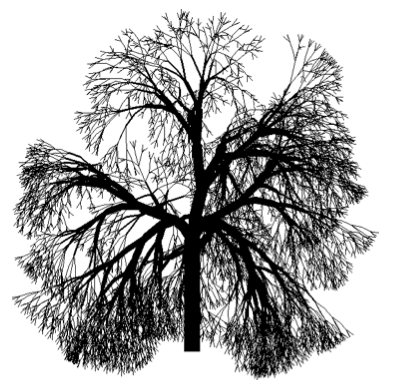
\includegraphics[width=.63\textwidth]{trees1.png}
    \caption{}
    % \label{fig:balanced}
  \end{subfigure}%
\end{figure}
\begin{figure}[H]
\ContinuedFloat
  \begin{subfigure}{.5\textwidth}
    \centering
    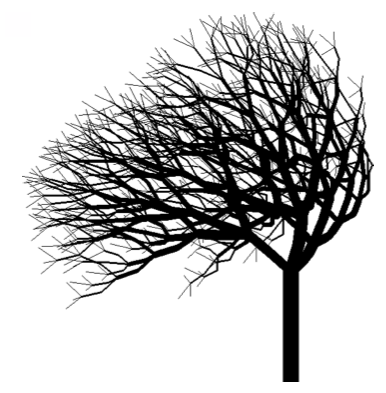
\includegraphics[width=.63\textwidth]{trees2.png}
    \caption{}
    % \label{fig:unbalanced}
  \end{subfigure}
  \caption{Examples of trees with ternary branching$^{\text{\cite{Prusinkiewicz:1996:ABP:235579}}}$}
   \label{fig:ttrees}\end{figure}

\section{Interdependence} % (fold)

\label{sec:interdependence}

Three dimensional parametric and stochastic L-Systems are a really powerful tool that help us model complex botanical structures such as monopodial, sympodial and ternary trees.By varying global parameters we can regulate some fixed parameters such as the way gravity affects the tree or the branching angle that the tree will follow. We can visualize these ideas in the ternary trees shown in Figure \ref{fig:ttrees}.

However, whereas we need stochastic systems as a source of variability to realistically emulate the structure of forests, there is a enormous caveat using them for multiple independent L-systems. To look into the problem lets consider the size of a state string $S$ as $|S| = L$. If each production rule translate one symbol into two and we only have deterministic production rules, the output will have size $2L$. However, if each production rule only substitutes with a $50\%$ chance then we only expect half of the symbols to change and the expected size of the output string will be $3L/2$. So we can find a proportionality between input and output sizes and this will deem an exponential growth. However, if by chance, one string gets a significantly greater or lower amount of successful production rules this will affect in the next iteration, since having more symbols in the string will allow the system to grow faster and viceversa.

This produces an oddly looking unrealistic system as we can see in Figure \ref{fig:stochas} where one of the plants has, after a few iterations has grown bigger, and will keep doing so; whereas other plants have carried average iterations resulting in similar systems. This phenomenon can be justified by the fact that: a) the systems are completely independent of each other and therefore do not share any common parameters, b) we are not taking into account any real model for the shared medium, such as mineral resources.

\begin{figure}[H]
  % \centering
    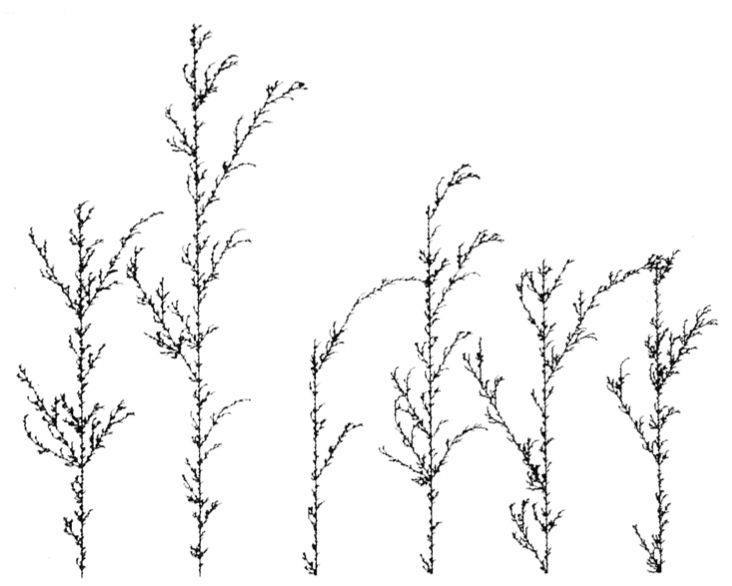
\includegraphics[width=.5\textwidth]{stochastic.png}
    \caption{Simulated growth of several simple stochastic L-Systems$^{\text{\cite{Prusinkiewicz:1996:ABP:235579}}}$}
    \label{fig:stochas}
\end{figure}

In a similar fashion as \cite{KurthSloboda2002} did, we can employ  both the global parameters to the system and universal parameters to the whole group of systems to thwart this undesired behavior. These parameters display the relationship between different systems or different parts of the same system, and are usually updated after each derivation step with the information provided by different metrics on the current string state.  Depending on the locality of the parameters we can differentiate two types of dependence:
\begin{compactenum}[a)]
\item \textbf{Selfdependence} - In this case there exists a relationship between different parts of the same system. For example, given a tree whose production rules depend on the amount of light received by each branch would need to update this information after each timestep considering the shadows projected by its own branches.
\item \textbf{Interdependence} - A more complex case that involves relationships between potentially different types of L-Systems, and that reflects a reciprocal interaction between them. We can extend the previous example, given a number of trees if we consider not only the shadow of a tree to itself, but the shadow projected from other trees we will have introduced a interdependence relationship into the growth simulation.
\end{compactenum}

 Independent and selfdependent systems provide a embarrassingly parallel problem, since each system can be analyzed without considering the others they can be treated as individual problems. The load balancing can achieved by a simple manager-worker scheme using a shared queue. However, interdependent groups of L-Systems can pose a nontrivial parallelization given appropriate constraints. For this paper we have used a local resource economy which translates in the following behavior. A tree will only be affected by the trees within a radius R, which from now onwards will referred to as his \emph{neighbors}. If a tree is bigger than the average size of their neighbors then it will be harder for it to grow at the next iteration, preventing the overgrowth behavior depicted in Figure \ref{fig:stochas}. If a tree is smaller than the average size of its neighbors, then it will more likely for it to grow in the next iteration, compensating the randomness in previous iterations. We need to use this constraints since as we explained before, whereas randomness is a good source of variability for the population, it deeply alters the growth rate of different systems leading to undesired and unrealistic behaviors.

 We still need to define what the \emph{size} of a tree means from an analytical viewpoint. We will use the concept of \emph{metrics}, functions when given as an input a list of parametric symbols, output a list of real valued parameters that reflect different aspects of the system. In our implementation the metric employed measured both the number of nodes (points where branching occurs) and leaves (terminal points of the system) to account for the dimensions of the tree.
\vfill
\columnbreak
 A serial implementation of the described scenario was carried out\footnotemark. A fixed number of different L-Systems composed a given probability distribution of monopodial, sympodial and ternary trees was randomly distributed in a square surface. All these tree systems where slightly modified from the Honda canonical definitions given in \cite{Prusinkiewicz:1996:ABP:235579} to accommodate for randomness in the growth. Next, a neighbor look-up list was initialized, since neighboring relations do not change throughout the simulation. For a fixed number $k$ of iterations, each system was applied the derivation procedure and its metric recalculated and stored in a global array. Then, before starting the next iteration, the growth parameter of each system was updated using the metrics from its neighbors.

 This implementation allows for huge variability of environments. Modifying the probability distribution of trees, the size of the Area, the number of systems and the number of iterations allow us to model from old, dense boreal forests to a widely spaced savanna.

\footnotetext{All the code for this project can be found in \href{http://github.com/JJGO/Parallel-LSystem}{http://github.com/JJGO/Parallel-LSystem}}

% section interdependence (end)

\section{Parallelization} % (fold)
\label{sec:parallelization}

When looking at a decently sized group of L-Systems ($N \approx 100$) and a considerable number of iterations ($k \approx 14$), the serial implementation starts taking seconds on most modern machines. Trying to increase any of the parameters goes to the domain of minutes and even hours. Therefore, the problem can use parallelization techniques in order to reduce the computation time by introducing more processing power. For this analysis we have chosen a shared memory architecture using the OpenMP application programming interface in C++. In this paper we are going to focus in the parallelization of the derivation step for the interdependant system described in Section \ref{sec:interdependence}.

The interpretation step of multiple L-Systems is an inherently embarrassingly parallel problem since all of the systems are independent when it comes to interpretation. To further optimize the parallelization of the interpretation step, one can look at parallelizing the interpretation of an individual L-System. This can be easily done for \emph{non-branching} systems by replacing each symbol with its associated affine transformation (4x4 matrix). Since matrix multiplication is an associative operation we can easily solve the problem by using a \emph{reduce} function. \emph{Branching} systems can follow a similar approach but the complexity escapes the scope of the current paper. A more  detailed explanation can be found in \cite{LIPP-2010-PGMS}.

\subsection{Dynamic scheduling} % (fold)
\label{sub:dynamic_scheduling}

% subsection dynamic_scheduling (end)

A initial naive parallelization can be used by just simply parallelizing each one of the derivation iteration steps. Using a dynamic scheduling algorithm, the processors will evenly split the work and solve each iteration in parallel. We consider dynamic scheduling instead of static scheduling to get a better load balancing scheme. Even though we know the amount of subproblems from the start, we cannot evenly divide them into the processors since the complexity of each system will be variable due to the  stochastic formulation that the trees are following. Dynamic scheduling will be dealt in a \emph{first-come, first-served} manner to optimize allocation

As we shall see later in Section \ref{sec:results}, this approach decreases the overall time but is far from perfect. The main disadvantage associated with this approach comes from the fact that an implicit barrier is set up at the end of each iteration to ensure correctness. This will imply that for $p$ processors and $N$ similarly sized trees, at the end of each iteration approximately $r \equiv N \mod p$ processors will be still working and $p - r$ will be idle, waiting for the rest to finish and wasting processing power. On average, this means that half of the processors will be idle for approximately $\frac{1}{\ceil{N/p}}$ part of the time. As $p$ grows larger this fraction also becomes larger which is undesirable. Furthermore, the presence of the two implicit \emph{barriers} per iteration produces a great overhead since all threads will be synchronized after each iteration. Therefore, we will need to reduce all of this communication to a minimum.

% subsection dynamic_scheduling (end)

\subsection{Lookahead strategy} % (fold)
\label{sub:lookahead_startegy}

Given the constraints of the problem we can enhance the parallelization by taking into account two factors:
\begin{compactenum}[a)]
\item \textbf{Local dependence} - As we explained before, the simulation has only a local dependence from a tree to its neighbors. Therefore, we need not wait for every tree to finish iteration $i$ to start iteration $i+1$. A given tree $t$ at iteration $i$ only needs the metrics of its neighbors at iteration $i$ to start the derivation phase. By applying this mechanism we can make use of every the processor available all the time; however, we will need to introduce series of constraints into the implementation.

An additional verification step must be performed to test if all the neighbors have in fact reached at least the current iteration and proceed only if the minimum of their iterations is bigger or equal the iteration of the system at hand.

The shared array that previously stored the metrics at each iteration will need another dimension for all the iterations, otherwise, we could potentially be reading a metric from a future iteration of a given neighbor, and correctness would be violated. Therefore, we will need to store for each tree $t$ the metric at every iteration $i$.

Since no two processors will try to update the same metric or iteration variable during the entire program and reading not yet updated iteration variables does not affect the correctness; we will not need mutual exclusion to modify the metric variables. Accordingly, the communication is clearly lessened to only the neighbor checking and the work scheduling.

\item \textbf{Geometry of the subproblems} - Since the simulation is running in parallel over all the $N$ trees for $k$ iterations we know in advance that $N \cdot k $ derivation steps will need to be done. We can dynamically schedule all this subproblems via an ordered work queue, so that the processors can take one subproblem at a time and if the derivation is possible (the neighbors have reached all the previous iteration) they will proceed, otherwise they will return the work to the queue and try the next available subproblem.

Since we are using an approach that relies on the connectivity of the trees in the forest, we can express the neighboring relationships as a undirected graph. An arbitrary queue will render a great amount of the neighbor checking steps unsuccessful, since we cannot predict which vertices have been derived yet and which not.

However, we can make use of the inherent geometry of the problem by employing a graph traversing algorithm such as \emph{Breadth First Search}. By performing an initial \emph{BFS} traversal into the graph and storing this precalculated order we can ensure that if at every iteration, the nodes are interpreted in the same order, then we will be maximizing vertices whose neighbors all have the same iteration value.

Consequently, the algorithm will start deriving at a given starting point of the graph and traversing it following BFS. When the other end is reached, a number of processors may not have work to do in said end, so they can go back to the starting point of the graph and  with a really high probability, they will be able to derive the next iteration of the vertices there, maximizing the processing power.

\end{compactenum}

With all this optimizations the program works almost as good as before (for some inputs the neighbor checking slows the algorithm) when $p \mid N$ and much better in cases where $N \mod p$ is really small which implies that for the previous implementation, a big fraction of the processors will be idle for an entire derivation step at the end of each iteration. Since the complexity of the derivation steps grows exponentially, this enhances the simulation runtime significantly.


% subsection lookahead_startegy (end)

\subsection{Connected components optimization} % (fold)
\label{sub:connected_components}

A further optimization can be made. The main disadvantage of the solution proposed in section \ref{sub:lookahead_startegy} comes from the fact that it introduces a whole neighbor checking phase that can consume a non-negligible amount of resources if the graph presents great connectivity. Also, the simulation uses as inputs both dense and sparse groups of trees in order to satisfactorily model different types of environments. This implies that in some cases we will have a single highly connected graph and in other cases we may have several smaller subgraphs or even individual vertices.

Moreover, as we briefly commented in the previous section the neighbor checking may be unnecessary in some cases. Specifically, when all processors are executing trees in the same iteration, neighbor checking needs not be done. By using a series of flag variables we can check if all the processors are in the same iteration and skip the neighbor checking.

In addition, to improve  the algorithm we can also use the fact that we are performing a initial BFS to compute a order of visit to the vertices and also identify the different connected components of the graph. This is useful, since connected components in the graph render completely independent subgroups of L-Systems that will not share any information whatsoever during all the iterations. Using this information we can split the main queue into smaller queues which helps reducing the overhead of scheduling the work.

% subsection connected_components (end)

\subsection{Splitting L-Systems} % (fold)
\label{sub:splitting_l_systems}

To try to extend the parallelization further an attempt was made to parallelize the derivation of individual L-Systems. This rendered a problem when either $N$ was really small or $k$ was exceedingly big. To successfully divide a L-System into smaller work items, we can use the fact that L-Systems are parallel rewriting grammars. Since all the L-Systems covered in this implementation are context free, we can just evenly divide the number of symbols in the system in $m$ different pieces and add them into the dynamic queue. It is important that they are not dispersed in the queue since as we analyzed before, the neighbor checking pattern works better when given a BFS order for the nodes. The L-Systems were slightly modified to cope with the multiple updates that now a derivation step needs to do. The iteration value will not change until the last derivation part is finished.

Following this scheme and building on top of the previous optimizations, we successfully reached a correct solution that split the work for L-Systems when idle processors are present and directly depend on that system to continue the work with another the derivation of another systems. However, the overhead involved in both checking if one L-System is bottlenecking the derivation and maintaining a queue with both entire L-System states and partial ones rendered the solution useless since it increases the serial time by at least one order of magnitude for almost all inputs. Consequently, this implementation was not used for the final results.

% subsection splitting_l_systems (end)

% section parallelization (end)

\section{Results} % (fold)
\label{sec:results}

To thoroughly test the parallelization, the parallelization techniques described in section \ref{sec:parallelization}, were implemented incrementally and tested independently. As data inputs we used a variety of tree models monopodial, system and ternary trees depending on the density properties of the forest. They all shared the same defining parameters, since forests are usually made of trees with similar characteristics. Randomness was employed to place the points in a plane. A square surface was used, whose size was randomly established at the beginning. The value for the size oscillated within the range $\sqrt{\sqrt{N}} \leq s \leq \sqrt{2N}$, since bigger sizes led to very sparse systems and smaller systems produced highly concentrated systems,  and neither of them resembled a realistic forest model. Therefore, by randomizing the area we are getting a random density for each testcase.

As we also explained in previous section randomness is a crucial part in the derivation of stochastic L-Systems. At the interpretation of every nontrivial symbol, randomness is used to decide between using the default production rule or the plain identity. This coupled with the interdependence strategy models the forest behavior as desired.

We made an analysis with numerous values for $N$ and $p$ and realized that in general, the strategies outlined in Section \ref{sub:dynamic_scheduling} and \ref{sub:lookahead_startegy} have significant improvement but the optimization outlined in section \ref{sub:connected_components} was only marginally better than \ref{sub:lookahead_startegy}. The last improved worked in less time for a really specific type of inputs and in general, the speedup was compensated by the added overhead.

Therefore, in the figures and plots we are going to differentiate between two cases, the initial algorithm with just sequential dynamic scheduling which will be denominated ``\emph{dynamic}'' and the one that takes the rest of the optimizations into account, which will be referred as the ``\emph{lookahead}'' algorithm. Since adult trees require between 11 and 14 iterations to ``grow'' we have used $k = 12$ for the forests. Now, for the input sizes, we have $N = 65, 110, 220$ which were reasonable values for formulated model.

\subsection{Timing results} % (fold)
\label{sub:timing_results}

The obtained timing results are gathered in Tables \ref{tab:Times_dynamic} and \ref{tab:Times_lookahead}. A great variety of number processor amounts were used ($1, 2, 4, 8, 16, 32$). Averages were taken in order to get uniform results for the different random inputs and to eliminate potential machine inefficiencies introduced in the execution of the program.

For a better understanding of the behavior of both algorithms for the data covered in both tables, the figures depicting timing results, SpeedUp and Efficiency are provided. (Figures \ref{fig:times}, \ref{fig:SpeedUp}, \ref{fig:Efficiency}).

\begin{table}[H]
    \begin{subtable}{.5\textwidth}
      \centering
        \begin{tabular}{*{7}{r}}
        $ N \setminus p$ &   \multicolumn{1}{c}{\textbf{1}} &\multicolumn{1}{c}{\textbf{2}} &\multicolumn{1}{c}{\textbf{4}} &\multicolumn{1}{c}{\textbf{8}} &\multicolumn{1}{c}{\textbf{16}} &\multicolumn{1}{c}{\textbf{32}}\\
            \midrule
            65 & 1.060 & 0.767 & 0.411 & 0.262 & 0.121 & 0.104 \\
            110 & 1.881 & 1.241 & 0.675 & 0.412 & 0.203 & 0.152 \\
            220 & 3.462 & 2.418 & 1.324 & 0.682 & 0.388 & 0.279 \\
        \end{tabular}
        \caption{Times for the dynamic algorithm ($k = 12$)}
        \label{tab:Times_dynamic}
    \end{subtable}%

    \begin{subtable}{.5\textwidth}
      \centering
        \begin{tabular}{*{7}{r}}
        $ N \setminus p$ &   \multicolumn{1}{c}{\textbf{1}} &\multicolumn{1}{c}{\textbf{2}} &\multicolumn{1}{c}{\textbf{4}} &\multicolumn{1}{c}{\textbf{8}} &\multicolumn{1}{c}{\textbf{16}} &\multicolumn{1}{c}{\textbf{32}}\\
            \midrule
            65 & 1.150 & 0.734 & 0.363 & 0.191 & 0.112 & 0.077 \\
            110 & 1.817 & 1.036 & 0.594 & 0.285 & 0.160 & 0.091 \\
            220 & 3.295 & 2.380 & 1.073 & 0.538 & 0.306 & 0.168 \\
        \end{tabular}
        \caption{Times for the lookahead algorithm ($k = 12$)}
        \label{tab:Times_lookahead}
    \end{subtable}%

    \caption{Timing results (in seconds) for both algorithms }
    \label{tab:Times}
\end{table}

As we can see in both Figures \ref{fig:times110} and \ref{fig:times220}, both algorithms successfully parallelize the problem. The \emph{lookahead} algorithm does on average always better roughly by a factor of two than the \emph{dynamic} algorithm.

\begin{figure*}
  \centering
  \begin{subfigure}{.5\textwidth}
    \centering
    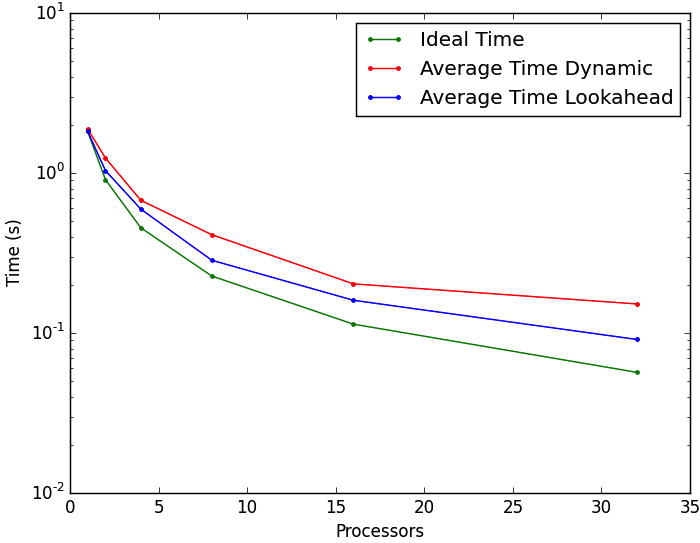
\includegraphics[width=.93\textwidth]{../3 Analysis/time_110.png}
    \caption{$N = 110$}
    \label{fig:times110}
  \end{subfigure}%
  \begin{subfigure}{.5\textwidth}
    \centering
    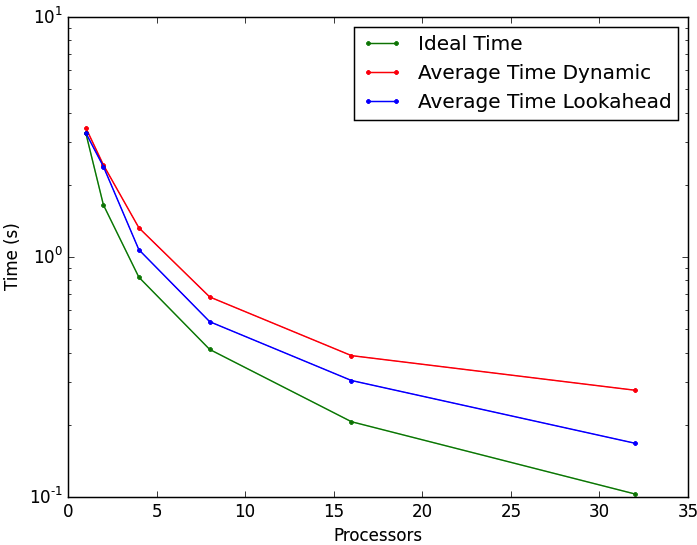
\includegraphics[width=.93\textwidth]{../3 Analysis/time_220.png}
    \caption{$N = 220$}
    \label{fig:times220}
  \end{subfigure}
  \caption{Logarithmic plot of times for different number of processors and inputs}
  \label{fig:times}
\end{figure*}

\begin{figure*}
  \centering
  \begin{subfigure}{.5\textwidth}
    \centering
    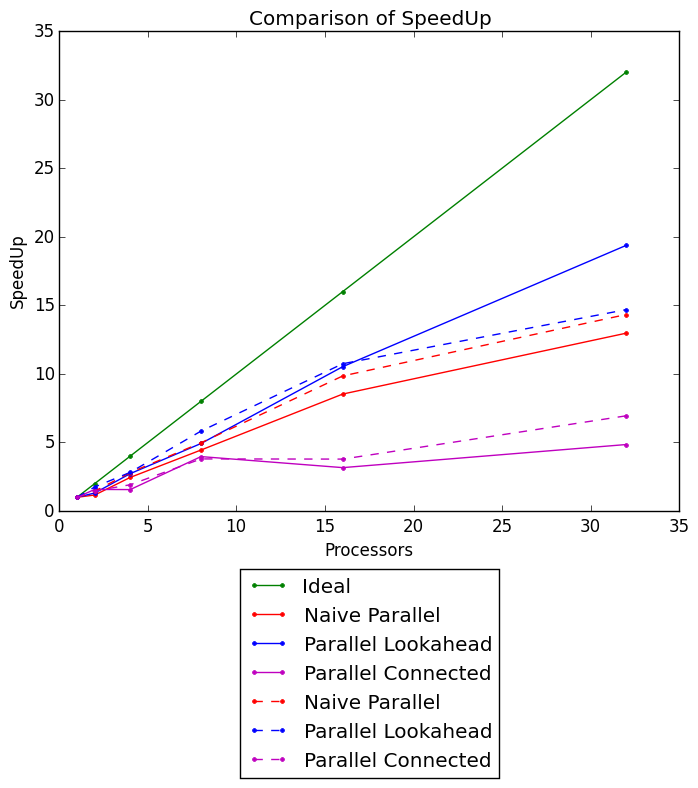
\includegraphics[width=.99\textwidth]{../3 Analysis/SpeedUp.png}
    \caption{Speed-Up}
    \label{fig:SpeedUp}
  \end{subfigure}%
  \begin{subfigure}{.5\textwidth}
    \centering
    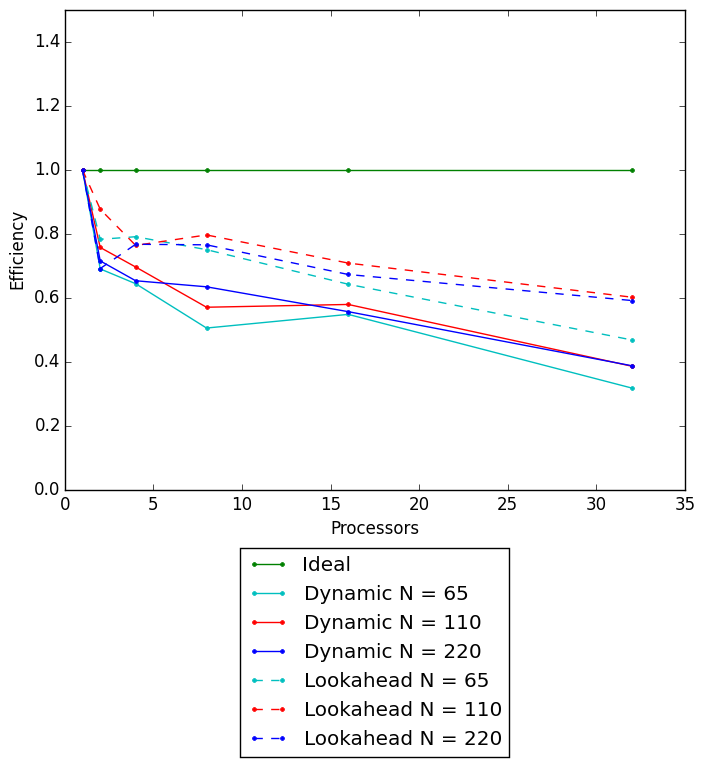
\includegraphics[width=.99\textwidth]{../3 Analysis/Efficiency.png}
    \caption{Efficiency}
    \label{fig:Efficiency}
  \end{subfigure}
  \caption{Speed-Up and Efficiency plots for the ideal case, Balanced and Unbalanced Workload}
\end{figure*}

\begin{table*}[t]
	\null\hfill
    \begin{subtable}{.45\linewidth}
      % \centering
        \begin{tabular}{*{5}{r}}
        \textbf{p} &  \textbf{ideal} & \textbf{average} &       \textbf{min} &       \textbf{max} \\
            \midrule
            1 &     1320.0 &    1320.0 &    1320.0 &    1320.0\\
            2 &      660.0 &     660.0 &     647.0 &     672.0\\
            4 &      330.0 &     330.0 &     315.0 &     345.0\\
            8 &      165.0 &     165.0 &     131.0 &     201.0\\
            16 &       82.5 &      82.5 &      47.0 &     137.0\\
            32 &       41.2 &      41.2 &      18.0 &     100.0\\
            
        \end{tabular}
        \caption{Load balancing of systems}
        \label{tab:Load_systems}
    \end{subtable}%
   	\hfill
    \begin{subtable}{.5\linewidth}
      % \centering
        \begin{tabular}{*{5}{r}}
        \textbf{p} & \textbf{ideal} & \textbf{average} &       \textbf{min} &       \textbf{max} \\
            \midrule
            1 &  1553837.0 & 1553837.4 & 1553837.0 & 1553837.0\\
            2 &   734333.5 &  734333.8 &  731044.0 &  737623.0\\
            4 &   365782.5 &  365782.7 &  360182.0 &  371576.0\\
            8 &   184617.5 &  184617.5 &  177446.0 &  191610.0\\
            16 &    96045.2 &   96045.3 &   88506.0 &  104027.0\\
            32 &    45396.5 &   45396.5 &   38811.0 &   54650.0\\
        \end{tabular}
        \caption{Load balancing of symbols}
        \label{tab:Load_symbols}
    \end{subtable}%
    \hfil\null
    \caption{Results for the load balancing analysis for $N = 110$ and $k = 12$}
    \label{tab:Load}
\end{table*}

Looking at the SpeedUp and Efficiency (Figure \ref{fig:SpeedUp} and \ref{fig:Efficiency}), we see that in fact the SpeedUp of the \emph{lookahead} algorithm behaves not only better than the \emph{dynamic} one, but also for a large enough input $N$, it gives a linear speedup. Bigger input sizes were also analyzed but the results obtained were almost identical to those for $N = 220$. For $N=65$ the SpeedUp is worse because the amount of work is not large enough to compensate for the communication overhead that the dynamic scheduling involves. The SpeedUp for the \emph{lookahead} algorithm is almost linear whereas the \emph{dynamic} algorithm presents a linear SpeedUp for $p < 16$ and greatly decreases for $p = 32$.

Efficiency analysis gives some interesting results. First for almost all of the testcases the efficiency is not strictly decreasing, which means that the algorithms are able to parallelize better for some specific values of $p$. However, we can see a decreasing trend for all of the cases, with the \emph{dynamic} decreasing faster than the \emph{lookahead} which agrees with the results of the SpeedUp.

% subsection timing_results (end)

\subsection{Load Balancing} % (fold)
\label{sub:load_balancing}

Load balancing measurements were taken for both algorithms, however, with the given inputs the results were practically indistinguishable (they both load balance correctly, the second algorithm is just able to do it faster), so we can just focus in whether the load balancing is happening correctly or not. We considered both the load balancing of systems and the load balancing of symbols and got averages of the average, minimum and maximum case in each scenario. We also computed the ideal load balancing by dividing the total number of symbols/systems by the amount of processors. This was all done for different $N$ but as with the algorithms, the results were identical so only $N = 110$ is provided as a matter of simplicity.

Again, for a better understanding of the gathered results, accompanying Figures are provided in \ref{fig:Load_systems} and \ref{fig:Load_symbols} that depict both the load balancing of symbols and systems in a logarithmic scale.

Using this figures and tables we can confirm that the dynamic scheduling approach proposed in Section \ref{sub:dynamic_scheduling} is satisfactory. Figure \ref{fig:Load_systems} reveals that systems are not being load balanced. This was expected, since one of the problems we faced in this implementation was that parametric stochastic L-Systems have a variable complexity and therefore dividing them evenly between the processors via static scheduling would give subpar performance. Due to this fact we can observe the inmense variability that minimum and maximum amount of systems offer, in order to accomodate for the variable complexity of L-Systems.

\begin{figure*}
  \centering
  \begin{subfigure}{.5\textwidth}
    \centering
    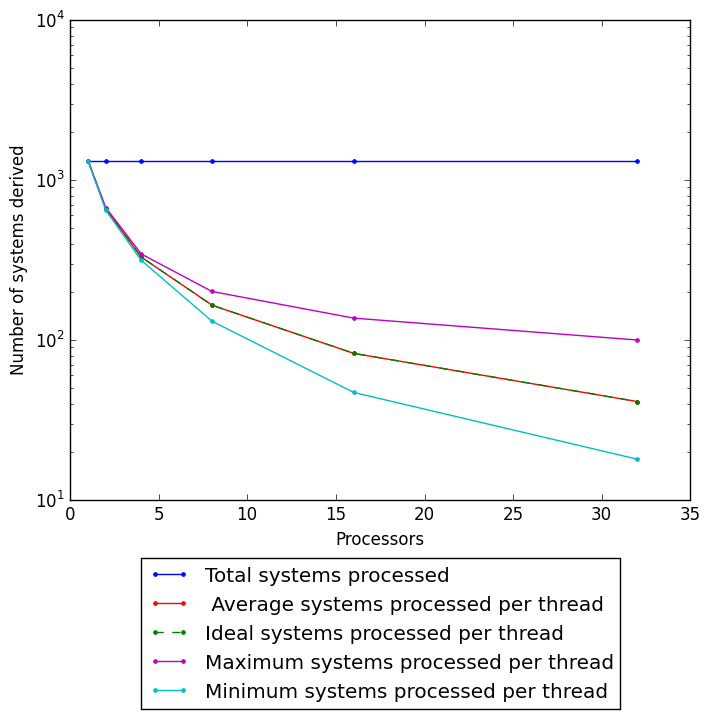
\includegraphics[width=.99\textwidth]{../3 Analysis/Load/systemsnaive110.png}
    \caption{Load Balancing of systems}
    \label{fig:Load_systems}
  \end{subfigure}%
  \begin{subfigure}{.5\textwidth}
    \centering
    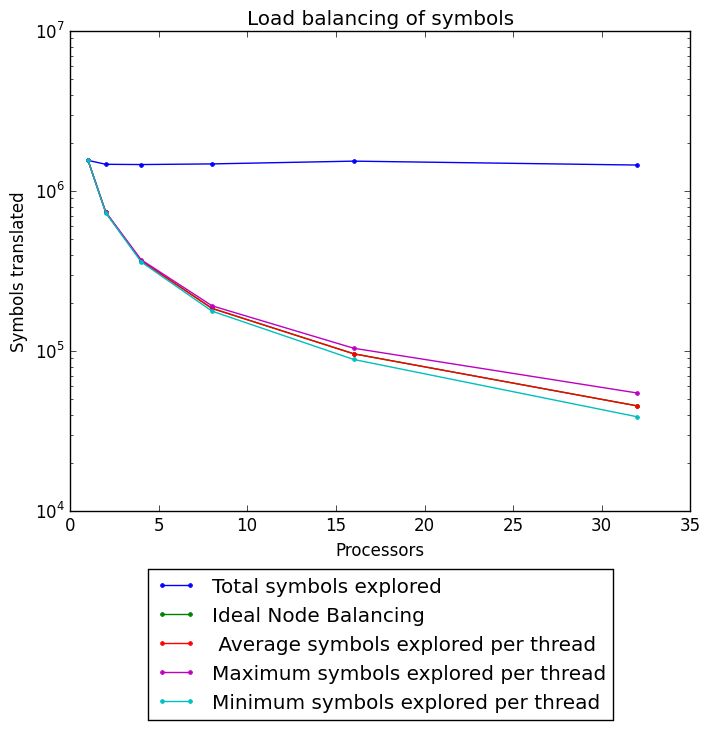
\includegraphics[width=.99\textwidth]{../3 Analysis/Load/symbolsnaive110.png}
    \caption{Load Balancing of symbols}
    \label{fig:Load_symbols}
  \end{subfigure}
  \caption{Results for the load balancing analysis for $N = 110$ and $k = 12$}
\end{figure*}

Figure \ref{fig:Load_symbols} truly indicates that load balancing is happening as expected and that all processors are doing an equal amount of work. In both figures we can appreciate that the ideal case is coincidental with the average case, but for symbol balancing we can see that maximum and minimum are extremely close to the ideal, suggesting that no processor is having a substantially larger or smaller amount of work.

% subsection load_balancing (end)

% section results (end)

\section{Discussion} % (fold)
\label{sec:discussion}

Multiple interdependent stochastic and parametric Lindenmayer systems are able to realistically simulate the growth behavior of a forest. Varying the L-Systems employed and the density of the trees allow us to model different types of environments, ranging from dense boreal forests to widely spread savannas. However, as with many procedural simulation techniques, the deriving cost comes at a price and if we want to simulate environments of considerable size, parallelization must be made to reduce the computing time needed.

From the results obtained in section \ref{sec:results} we can conclude that the parallelizing was successful and linear speedup was achieved for the final algorithm outlined in section \ref{sub:connected_components}. It is important to note that as $N = 65$ showed, the speedup will only hold if the input size is big enough for the amount of processors used. This is a fundamental characteristic of this problem. As with almost any type of parallelization, the communication will suppose the biggest burden to speedup and efficiency. In this particular problem, the communication is dealt via the dynamic scheduling algorithm described in section \ref{sub:dynamic_scheduling}. This involves a nontrivial amount of interaction between the processors. Furthermore, timing profiling for the execution revealed that we cannot easily increase the Speedup shown in Figure \ref{fig:SpeedUp} because time needs to be spent correctly scheduling the work. Otherwise, in a static scheduling, the complexity variability of the L-Systems completely spoils the load balancing and the results are far worse.

It is also important to mention that several other values of $k$ were tried for different input sizes and number of processors. As we explored in section \ref{sub:lookahead_startegy}, the plain dynamic scheduling behaves worse for larger values of $k$. However, for the cases when the difference was significantly bigger ($k > 16$), the model was overconvoluted and did not reflect any more the true appearance of a forest. Because of this, the results have not been analyzed. Albeit helping the case for the look-ahead algorithm, they do not represent a realistic scenario.

In conclusion, both the dynamic scheduling and the look-ahead strategy based in the BFS traversal have proved to be successful strategies to tackle the parallelization of the simulation. The connected components derivation just enhances marginally the behavior without adding a significant amount of overhead into the algorithm.


% section discussion (end)

\section{Conclusion} % (fold)
\label{sec:conclusion}

This report explores the viability of using parametric stochastic interdependent Lindenmayer systems to model the growth behavior of a forest, and a nontrivial way of parallelizing the problem. The final parallelization scheme involved a number of components which include a dynamically scheduled queue, an initial traversal search to determine the order of the nodes, a neighbor checking algorithm that deserialized the iteration steps allowing multiple iterations happen at once and finally a decomposition of the graph into smaller subgraphs to further optimize the results.

An important conclusion that we can gather from the analysis given is the fact that the nature of the L-Systems structure was not directly used in the parallelization (except for Section \ref{sub:splitting_l_systems}, which was unsuccessful). This means that the obtained parallelization algorithm can adequately model similar problems of the same characteristics. Namely, given a simulation problem with local dependence, and problems that grow with the same complexity after each iteration; the present algorithm should render similar results with comparable inputs, even if the internal elements are not precisely L-Systems.

\textbf{Future work:} The main caveat of the produced outputs was that all trees had the same ``age'', which translates in similar complexities (within one order of magnitude). This scenario is not unrealistic, (forest after fires develop in this fashion), but is far from general. We would like to analyze how the system would grow if new trees had the possibility to develop at any given iteration when certain circumstances are met, like the presence of neighboring trees. This would be an interesting problem to analyze, since adding this constraint breaks the main approach of the current parallelization.

In addition, the neighboring relationship was an absolute one, either two trees were neighbors or not. Reality is not discrete in this regard so we could further enhance the simulation by taking into account the distance as part of the relationship and defining a maximum distance for neighbors. Furthermore, as trees grow larger we could increase this radius to satisfactorily model the interdependence between the trees. Both of this additions would affect the parallelization scheme which would need to be rethought for these considerations.

% section conclusion (end)


%----------------------------------------------------------------------------------------
%	REFERENCE LIST
%----------------------------------------------------------------------------------------
\nocite{*}
\bibliographystyle{alpha}
\bibliography{mybib}
% \begin{thebibliography}{99} % Bibliography - this is intentionally simple in this template

% \bibitem[Figueredo and Wolf, 2009]{Figueredo:2009dg}
% Figueredo, A.~J. and Wolf, P. S.~A. (2009).
% \newblock Assortative pairing and life history strategy - a cross-cultural
%   study.
% \newblock {\em Human Nature}, 20:317--330.
 
% \end{thebibliography}

%----------------------------------------------------------------------------------------

\end{multicols}

\end{document}
